\chapter{User Manual}

This appendix explains the project operation by running the ``Scenario 1:
Emergencies-Lorca Earthquake'' defined in appendix~\ref{anex:scenarios}. To
execute it the experimenters must create an account in the \emph{Fed4FIRE} platform
and after that, they can already run the experiment. Then, the \emph{Rspec} of the nodes in
\vw is obtained from \emph{JFed}. The \ac{GUI} provides an
automatic manner to execute the experiment.

\section{First steps}
\label{sec:first-steps}
To experiment with the \emph{Fed4FIRE} testbeds, the following steps have to be
done (for more information, see \url{http://doc.fed4fire.eu/}): 
\begin{itemize}
\item To create an account in \emph{Fed4FIRE} in order to get some certificates
  to access testbeds.
\item To create an account in \bonfire for getting access in this testbed. At
  this moment, in order to use \emph{BonFIRE}, the experimenters also need to register for an additional account. 
\item To create an \ac{SSH} key and upload it in both the \emph{Emulab} and the
  \bonfire account.
\item To download the X.509 certificate which authorizes and authenticates the
  in all the \emph{Fed4FIRE} tesbeds.
\end{itemize}

\subsection{Creating a Fed4FIRE account}

The \emph{Fed4FIRE} webpage for creating an account is available in
\url{http://www.wall2.ilabt.iminds.be}. Once the page was loaded, the user has
to select the option ``Request an Account'' which is located on the middle of the page.

\begin{figure}[!h]
\begin{center}
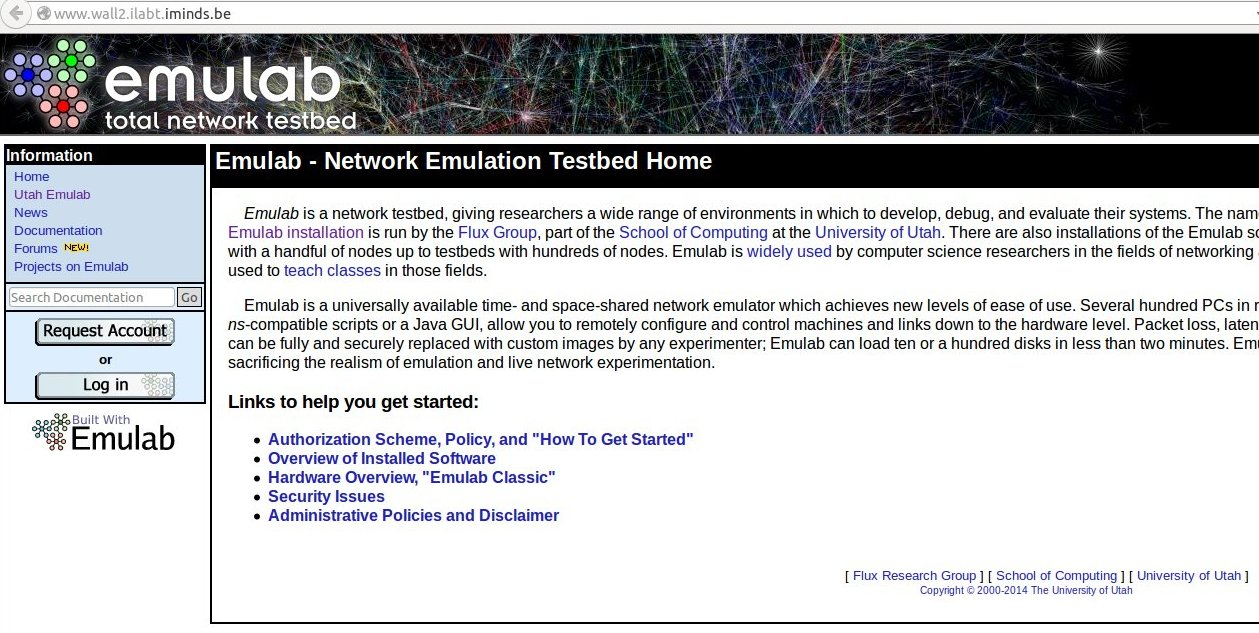
\includegraphics[width=0.7\textwidth]{user-manual/emulab.jpg}
\caption{Fed4FIRE webpage for creating an account}
\label{fig:fed4fire-account}
\end{center}
\end{figure}

Then, the experimenter must fill the registration form and to click in the ``Submit''
button. The account is created and it shall be validated by the \emph{Fed4FIRE}
reviewers. 

\subsection{Creating a BonFIRE account}

To a \emph{BonFIRE} account, the experimenter has to visit the platform webpage
\url{http://portal.bonfire-project.eu/}. Then, the experimenter fills the
registration form and sends it for approving. 

\begin{figure}[!h]
\begin{center}
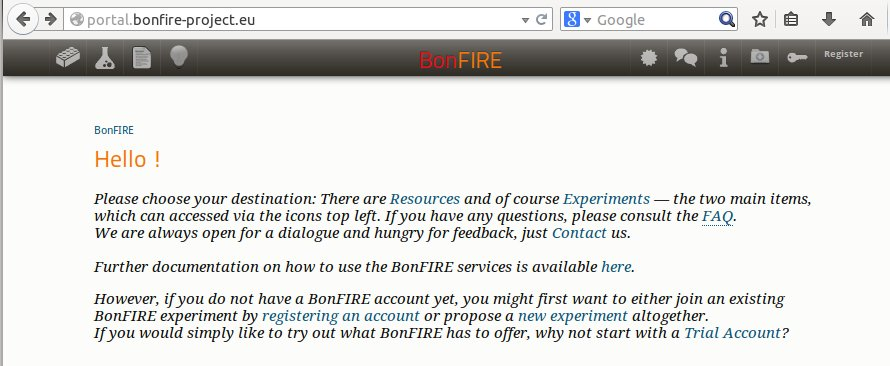
\includegraphics[width=0.7\textwidth]{user-manual/bf.jpg}
\caption{BonFIRE platform webpage}
\label{fig:bonfire-account}
\end{center}
\end{figure}

\subsection{Creating an SSH key}

Once the experimenter is registered in the \emph{Fed4FIRE} platforms, it is
necessary to create a pair of \ac{RSA} keys and to upload the generated public key to
\bonfire and \emph{Fed4FIRE} web plattforms. The creation of the \ac{RSA} keys,
depending on the operative system, can be done as follows:
\begin{itemize}
\item \emph{Windows platforms}: \emph{Putty} can be used. \emph{PuTTY} is a widely
  used \ac{SSH} client for Windows and it includes the tool \emph{PuTTYgen} to create
  an \ac{SSH} key. \emph{PuTTY} can be downloaded from
  \url{http://www.chiark.greenend.org.uk/~sgtatham/putty/download.html}.

\item \emph{Unix platforms}: For UNIX platforms, creating an \ac{SSH} key can be
  done through a command line tool in a terminal. The command that
  performs that is the following: \emph{``ssh-keygen -t rsa''}.

\end{itemize}


\section{Execution of a Scenario}

The prerequisites for a experimenter can perform the execution of a scenario are
the following:
\begin{itemize}
\item The \sss is running in the \vw testbed
\item To execute the software of cloud components. 
\item To execute the \ac{GUI} to manage the execution.
\end{itemize}

\subsection{Execution of the Satellite System Simulator in Virtual Wall}

To start the execution of the \sss in \vw, it is neccesary to do the
implementation as the Section~\ref{sec:impl-vw} explains.

Firstly it is necesary to obtain the \emph{Rspec} of the deployed nodes in
\emph{JFed}. Openning \emph{JFed}, the specification is located in
``source/vw/Description.rspec'' (see Figure~\ref{fig:loading-rspec}). Then, the Rspec is shown in
the window as the Figure~\ref{fig:rspec} shows.

\begin{figure}[!h]
\begin{center}
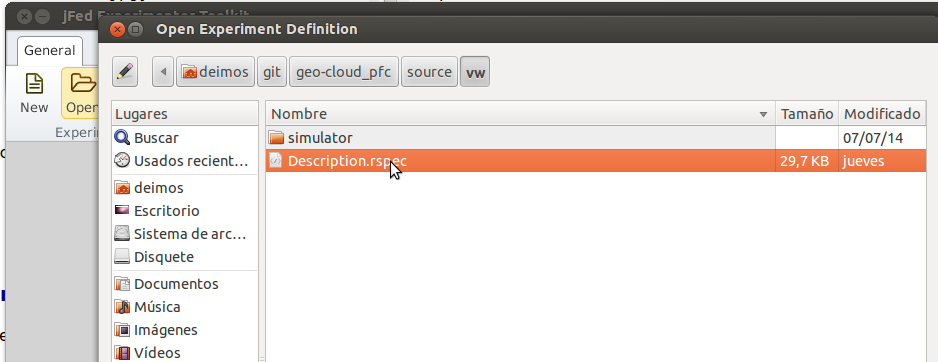
\includegraphics[width=1.0\textwidth]{user-manual/open-description.png}
\caption{Loading specification in JFed}
\label{fig:loading-rspec}
\end{center}
\end{figure}


\begin{figure}[!h]
\begin{center}
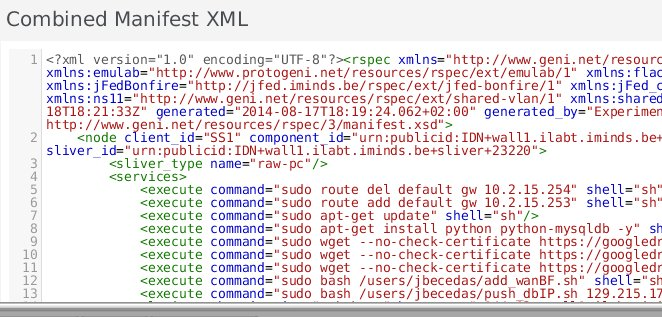
\includegraphics[width=0.7\textwidth]{user-manual/rspec.jpg}
\caption{Rspec in JFed}
\label{fig:rspec}
\end{center}
\end{figure}


The execution of the \sss is executed by clicking of the \emph{Start} button of
the \emph{JFed} interface. Thus, the experiment is executed (see Figure~\ref{fig:running-jfed}).

\begin{figure}[!h]
\begin{center}
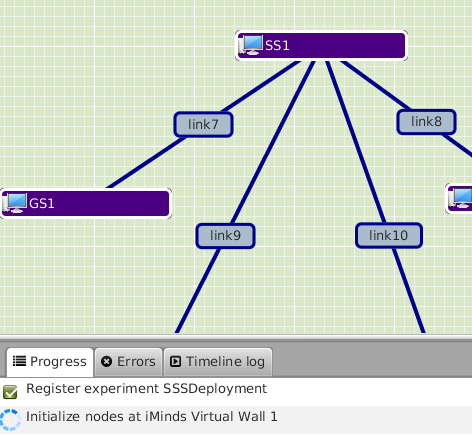
\includegraphics[width=0.5\textwidth]{user-manual/inicializando.png}
\caption{Running experiment in JFed}
\label{fig:running-jfed}
\end{center}
\end{figure}

At the end, all the nodes of the \sss are deployed and ready to execute the
software by using the \emph{GUI} (see Figure~\ref{fig:deployed-jfed}).

\begin{figure}[!h]
\begin{center}
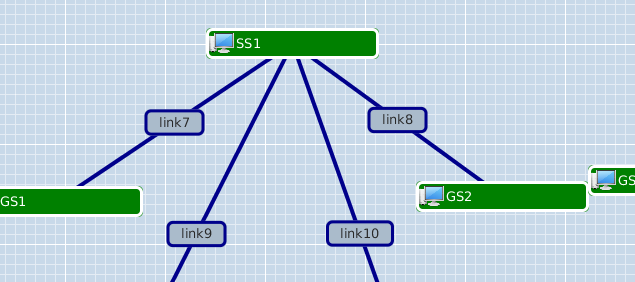
\includegraphics[width=0.7\textwidth]{user-manual/ok.png}
\caption{Nodes deployed in JFed}
\label{fig:deployed-jfed}
\end{center}
\end{figure}


\subsection{Execution of the Cloud Architecture in BonFIRE}

The execution of the cloud components are done as the
Section~\ref{subsec:ssh-cloud} shows. 
As summary, the orchestrator file config has to be configurated with the
\emph{Processing Chain} machine address, the database address and the \emph{Archive and Catalogue}
machine address. Then, the \emph{GeoServer} software in the \emph{Archive and
  Catalogue} machine is required in order to the Orchestrator can be
executed. Then, the \emph{Orchestrator is executed} (see Figure~\ref{fig:orch-execution}) and the
other components of cloud are executed on demand as soon as the
\emph{Orchestrator} requires them for processing images and archiving and
cataloguing them.

\begin{figure}[!h]
\begin{center}
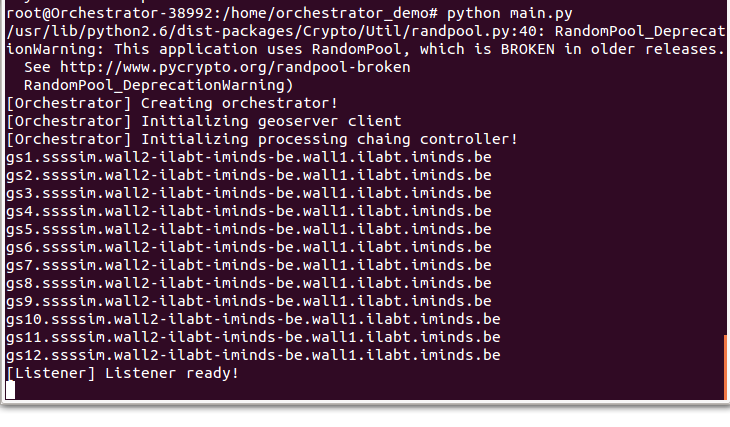
\includegraphics[width=0.8\textwidth]{user-manual/orchestrator.png}
\caption{Orchestrator execution}
\label{fig:orch-execution}
\end{center}
\end{figure}


\subsection{Execution of the GUI}

Once the cloud architecture  and the \sss are running respectively in \bonfire
and \vw and their setups were done, the system is ready for executing the
scenarios described in Annex~\ref{anex:scenarios}. The scenario selected in order to explain this
section was  the ``Scenario 1: Emergencies-Lorca Earthquake''.


The Figure~\ref{fig:rspec} shows the \emph{Rspec} specification which the user
has to fully select and copied into the ``gui/resources/jfed.out'' file,
replacing its content.

The next step is to execute the graphical user interface for experimenting. The
GeoCloud \ac{GUI} can be executed as ``python main.py'' in the main directory of
the \ac{GUI} ``source/gui''. Before that it is necessary to copy the
\emph{Rspec} specification of the \emph{JFed} when the experiment is
running. This is because the \emph{Experiment Controller} component of the
\ac{GUI} 

The main window appears and the experimenter can select the required scenario.
\begin{figure}[!h]
\begin{center}
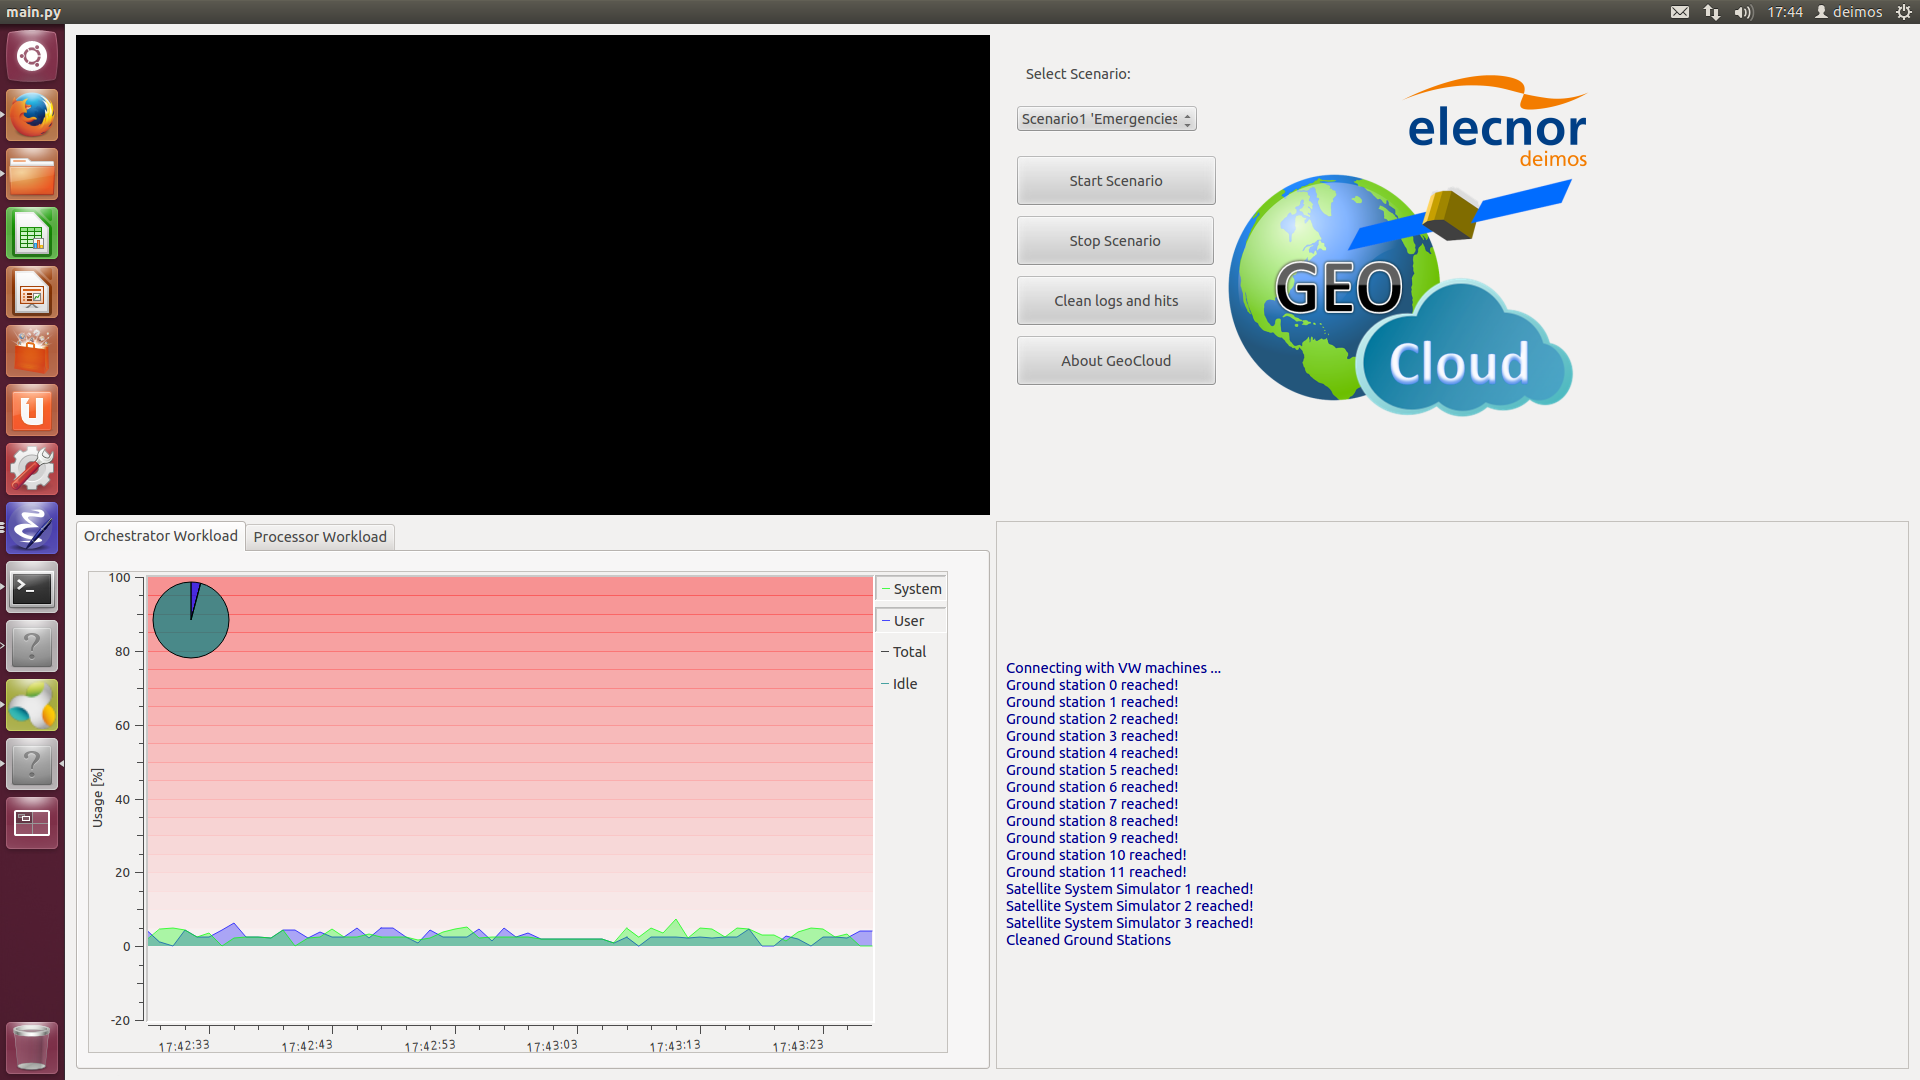
\includegraphics[width=1\textwidth]{user-manual/gui.jpg}
\caption{GUI main window}
\label{fig:gui}
\end{center}
\end{figure}

When the experimenter clicks the start button, the scenario begins to run and
the following actions are carried out: in the Log framework, several messages indicating the state of the execution
appear; in the Workload framework, it is displayed the workload of both orchestrator and
processing chain machines; and in the Video framework, the simulation of the
satellite constelation is displayed.

During the scenario execution, the acquired images from the satellites are processed
in the processing chain machine and sent to the catalogue. 
In the end, these images are available
in the web service provided by the \emph{Archive and Catalogue} module of the
cloud. 


\begin{figure}[!h]
\begin{center}
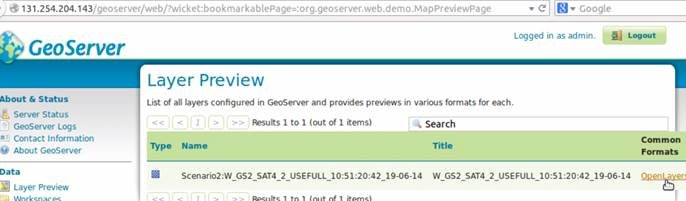
\includegraphics[width=1\textwidth]{user-manual/geoserver-capture.jpg}
\caption{GeoServer catalogue}
\label{fig:images-catalogued}
\end{center}
\end{figure}


\subsection{Collection of the results}

While a scenario is executing, the \emph{Orchestrator} is receiving all the
interactions that in the cloud system are carrying through. 
Basically, the experimenter has to connect to the \emph{Orchestrator} machine
and to get the ``orchestrator.log'' file for obtaining the experiment results.
This file contains the interactions produced in the system time stamped.
